Some of the same constraints developed in the field of solar-fuels apply to the case of solar fertilizers; however, there are also a number of new considerations which contribute to technological decision making. For instance there are two approaches to make renewable fertilizers. In the first approach, fertilizer manufacturing occurs through a nitrogen reduction process driven (indirectly or directly) by solar energy (renewable ammonia). In the second approach, solar energy drives the production of chemical feedstock’s for the Haber-Bosch process (renewable hydrogen)  (Fig. \ref{fig:reactor}). Another consideration is the low required solar-fertilizer efficiency requirements (when compared with solar-fuels), and the low volatility of products. The final considerations for solar-fertilizers is associated with the desired production location.  While most solar-fuels technologies are envisioned to operate in an industrial setting, there is strong motivation for solar-fertilizers technologies to operate in decentralized locations or at an agricultural site. \hl{While a detailed technoeconomic analysis is beyond the scope of this work, we present some general considerations for each approach.maybe this is misplaced-mch}

\hl{Include a figure here similar to the figures in solar fuels papers (e.g. Nate Lewis' work) comparing these two approaches}
\begin{figure}
    \centering
    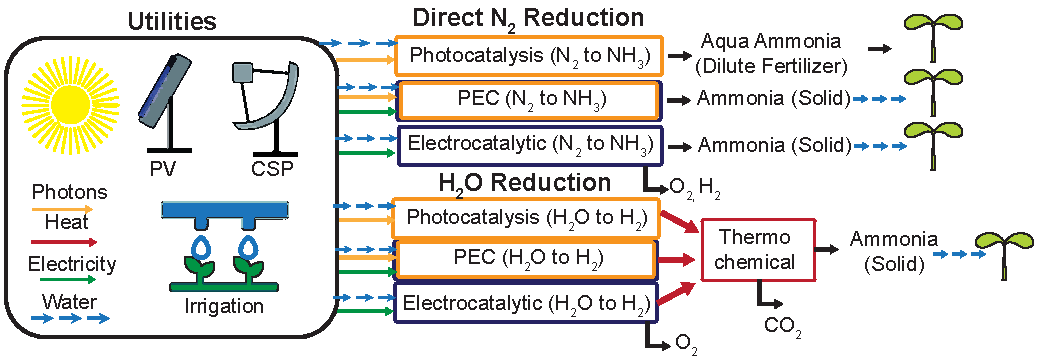
\includegraphics[width=1\textwidth]{Figures/Reactors.pdf}
    \caption{Schematic for solar fertilizer production. Solar fertilizer feedstocks include N\textsubscript{2}, H\textsubscript{2}O or H\textsubscript{2} and solar energy. }
    \label{fig:reactor}
\end{figure}
The direct capture of photons and conversion to fertilizer (renewable ammonia) is the most straightforward route to produce fertilizers at decentralized locations. Direct capture requires the use of a single catalytic material (or composite catalyst). Mass production and distribution of catalyst at low costs is also essential for widespread adoption. It is possible to envision relatively simple reactor designs that integrates directly with an irrigation system. Direct integration within an irrigation system, reduces operational complexity, and costs. These systems must operate without toxic electrolytes, avoiding the need for an additional energy intensive separation processes, and opening the possibility of inexpensive solar fertilizer reactors that could be deployed at the farm scale. However, the concentration of nutrients will be limited by the solar flux, leading to substantial uncertainty and likely lower concentrations (below the desired 1\%). Furthermore, photochemical technologies are relatively untested, and there is currently no catalyst capable of the required solar-to-ammonia efficiency of 0.1 \%. The most widely-used photocatalysts are for environmental applications such as reducing contamination or self-cleaning glass where concentrations are low and catalysts are inexpensive\cite{Bhatkhande_2001,Parkin_2005}. It is possible to envision solar fertilizer schemes that are similar to these environmental applications, but they would likely require close integration with agricultural infrastructure. For example, farms where irrigation is heavily employed are good candidates for direct solar fertilizers, particularly if they are located in remote regions. Roughly 7\% of farms in sub-Saharan Africa make use of irrigation. This is far from a majority, but still represents a substantial agricultural footprint where direct photochemical fertilizers might have a practical impact. \needcite

Electrochemical processes also require electrolytes to provide electrical conductivity and control the pH. Some reports have indicated that Li-based electrolytes exhibit high performance for electrocatalytic nitrogen reduction to ammonia\cite{Song_2018,Mikosch_2005}. In general the effect of electrolytes on plant growth are unknown, and some electrolytes that contain metals such as Li can be costly, indicating that separation of electrolytes may be required. On the other hand, many electrolytes such as NaCl are abundant and non-toxic, while others such as KOH and Na$_2$H$_2$PO$_4$ could provide an additional source of nutrients if they are not separated. Nonetheless, the need to deal with electrolytes introduces an additional engineering challenge. These intensive production processes would lead to higher capital costs and more centralized production; in this case issues with fertilizer transport would become relevant. As centralization increases the process will be in more direct competition with the established Haber-Bosch process, and more detailed technoeconomics will be necessary to determine if such an approach is competitive. Nonetheless, the scale of electro-chemical processes is still expected to be orders of magnitude below Haber-Bosch, and the process is likely to be less capital-intensive and more robust to uncertainty in electrical power. This suggests that agricultural areas in developed countries, near medium or large cities, or in land-locked areas are most promising for indirect capture of solar energy and subsequent electro-chemical conversion to fertilizers.

\hl{Add a table here with properties/advantages/disadvantages of direct vs. indirect?}

\subsection{Proposed process designs}

\begin{figure}
    \centering
    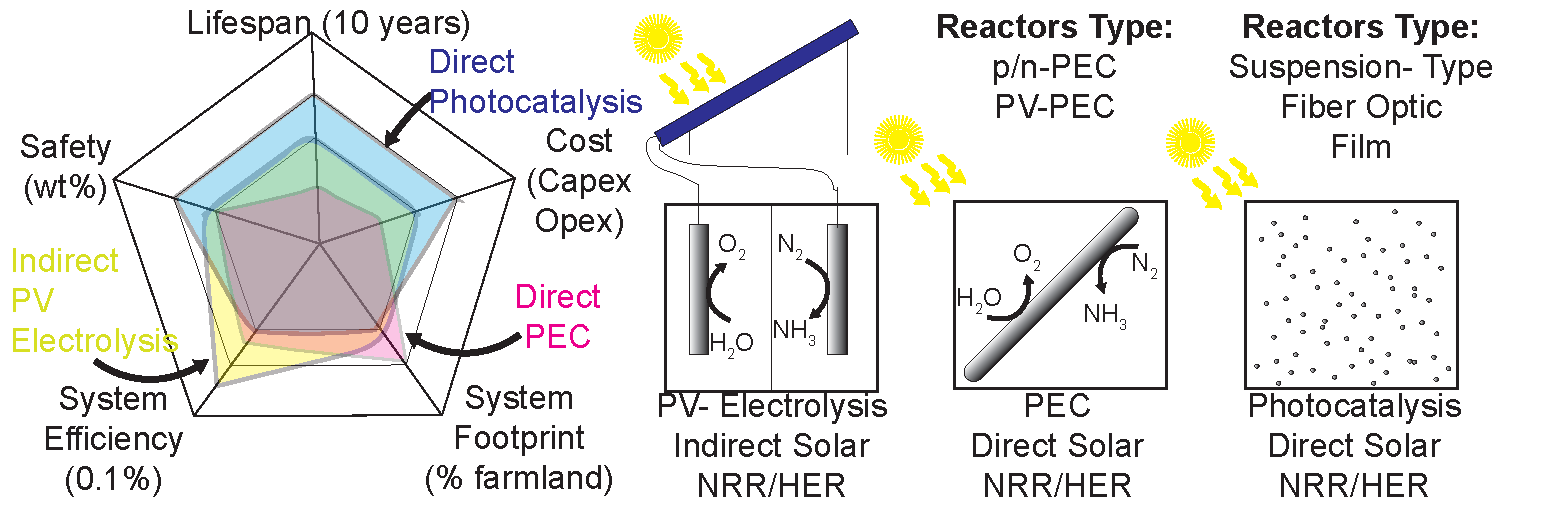
\includegraphics[width=1\textwidth]{Figures/Systems.pdf}
    \caption{}
    \label{fig:systems}
\end{figure}

 Briefly below we outline potential system architectures for solar-fertilizers, with an emphasis on discerning their cost (capitol and operational), efficiency, safety, and size.

\subsection*{Direct approaches for solar-fertilizers}

While there are currently no photocatalytic chemical production processes operation at scale, there exists a strong literature on photochemical reactor design for environmental applications and solar-fuel production.\cite{Mckone_2013,Birnie2006,walter_2010} It is likely, that the same principles and strategies will apply to the production of solar fertilizers. One reactor type heavily investigated is the suspension type reactor. A notable challenge with suspension type particles is the mixing of reduced and oxidized species (oxygen, ammonia and hydrogen), and the need to separate the two gas phase species. Despite these challenges, it is projected to be the cheapest approach to solar-fuel production.  In addition, there are  The first requirement of a photocatalytic reactor is to have an immobilized photocatalyst over which fluid can flow to prevent loss of catalyst. In practice, the photocatalyst is applied as a coating on a transparent material. Two common designs in commercial applications are flat plates\cite{Brandi_1999} and fiber glass cloths\cite{Horikoshi_2002} coated in photocatalyst. Reactors involving honeycombs of catalyst with embedded optical fibers to convey light have been proposed for CO$_2$ reduction photocatalysis.\cite{Ola_2015} These are all viable in principle for N$_2$ reduction, though capital costs and durability may be factors in the eventual viability of a given design.

Due to the low rates of reaction in current generation photocatalysts, a successful reactor design will likely be either a stagnant tank solar collection system or a low flow reactor, similar to a continuously stirred tank reactor (CSTR.) The photocatalyst could be either immersed in water or suspended above water to perform the reaction in an aqueous phase or gas phase respectively. The produced ammonia be kept at a high concentration within the reactor to maintain a high product concentration. In the case of using activated carbon as an adsorbent, the carbon would be suspended above the liquid to allow the gaseous products to diffuse into the pores in the gas phase.

Coupled solar capture/electrocatalysis systems are able to be more centralized than their photchemical analogs. A standard system may look similar to a membrane reactor from a chloralkali process, with flow cells consisting of electrodes separated by a semi-permeable membrane arranged in arrays.\cite{} These would be positioned near solar farms in rural areas. These could produce an aqueous solution of ammonia, which would be delivered in pipelines or by truck to nearby farms. Another possibility is coupling a biochar production facility with an electrochemical nitrogen system. The ammonia could be produced and concentrated in a bed of biochar. The biochar would then be delivered to local farms via truck or rail connections to be applied as fertilizer. Given that biochar facilities are already economically promising, the latter option may prove exceptionally attractive.\cite{Galinato2011}

\subsection*{Indirect approaches for solar-fertilizers (Photovoltaic-Electrolysis)}

Coupled Photovoltaic/electrochemical systems are currently more efficient than the photochemical approaches. However, some of the common reactor configurations require higher initial capital investment than photochemical approaches, due to the cost of the reactor components (membranes and catalysts). Electrolysis systems may be promising for use in small/medium ammonia manufacturing plants in a semi-decentralized manufacturing model. The largest challenge with the electrolysis systems is that there are no selective catalysts capable of reducing dinitrogen. The three prominent approaches which could be employed include alkaline based electrolyzer, proton exchange membrane (PEM) electrolyzer, and solid oxide based electrolysis (SOEC). 

\todo{need appropriate citations}Alkaline electrolysis cells operate in with a basic electrolyte (usually KOH or NaOH), and have achieved achieved efficiency's of 50\%-60\% and current densities of 100-300 mA/cm$^2$ for hydrogen production. PEM electrolyzers use a polymer membrane (Nafion) as a solid electrolyte, and have demonstrated efficiencies between 55\% and 70\% and current densities higher than 1600 mA/cm$^2$. And solid oxide electrolysis (SOECs) which operate in the mid temperature range (100-200 $^\circ$C) are able to achieve higher efficiencies (85\%-90\%). Unfortunately, the performance of current state of the art electrolysis cells do not translate to nitrogen reduction based electrolysis systems. 

The materials used in these reactors are costly because of the high temperatures that have to be withstood during the reaction. The biggest issue with SOECs is that the technology is still in early stages of development and sealing and corrosion problems are common. Due to the high initial capital investment, high efficiency, and high temperatures these reactors would be best used in large scale plants. 

\end{comment}

In addition to efficiency it is also critical to consider the concentration of fixed nitrogen needed for a product to be considered a fertilizer. The limiting case can be determined by assuming that the nutrients will be included directly in the irrigation lines. However, the amount of irrigation needed is highly variable depending on crops, rainfall, location, and socioeconomic factors (http://www.fao.org/docrep/u5835e/u5835e04.htm). Nonetheless, we propose an estimate of 1500 L/ha/y as a typical number for practical scenarios. Further, we note that while 50 kg-N/(ha yr) is a typical nitrogen nutrient load, the critical lower boundary for nutrient consumption can be as low as 15 kg-N/(ha yr). From these estimates we propose a lower boundary of 1 kg-N/L, or 1 wt \% N, as a convenient estimate for the minimum nitrogen concentration that can be considered a fertilizer \hl{compare to aqua ammonia and potential get insight from IFDC on what the potential impact might be of these low loads. Any previous experience where aqua ammonia is used for direct application?}. This is roughly 1 order of magnitude lower than existing aqueous fertilizers, but it is 5-8 orders of magnitude above the concentrations reported for typical photo(electro)chemical nitrogen fixation processes where yields are typically reported in units of $\mu$M or mM. This large gap between the proximity of efficiency and concentration targets is due to a combination of large water volumes and the short testing times that are typically employed for photo(electro)catalysts. Photocatalytic ammonia production is often measured in the gas-phase, where ammonia sticks to the catalyst surface and must be removed through water or heat, leading to low concentrations, and in aqueous photo(electro)chemical settings the fluid volumes are typically on the order of 100mL while illumination areas are on the order of cm$^2$. Furthermore, testing times on the order of days to weeks are considered long by academic standards. This leads to extremely low concentrations that are outside of the regime that can be considered fertilizer. Operating the catalysts in higher ammonia concentration regimes may impact the performance of the process, suggesting that future efforts should focus on designing cells and testing procedures that lead to substantially higher concentrations. These higher concentrations lead to an additional advantage for analytical characterization, since difficulties in quantifying ammonia at nM - $\mu$M concentrations have plagued the field. As concentration increases the issues with contamination will be less prevalent, and the presence of ammonia should become unmistakable due to its pungent odor that can be detected with concentrations of about 50 ppm\cite{Leonardos_1969} (equivalent to 3 mM in the aqueous phase).


current densities that are required for practical operation. In the case of solar fuels the overpotential for oxygen evolution has been defined as the potential at which the current is equal to 10 mA/cm$^2$, equivalent to 10 \% solar-to-fuel efficiency. In the case of solar fertilizers the necessary current will be substantially lower, due to the substantially lower solar-to-ammonia efficiency requirements. For simplicity, we will assume that a 0.1\% solar-to-ammonia efficiency is required. However, an additional consideration that is more relevant for electrochemical nitrogen fixation is the Faradaic efficiency that governs the selectivity to ammonia (or nitrates) over other possible products. Indeed, low selectivity to ammonia due to hydrogen evolution has proven to be a critical challenge for electrochemical ammonia synthesis.\cite{Singh_2017} Typical reported ammonia selectivities are $<$ 1\%, although several recent reports have achieved Faradaic efficiencies on the order of 10 \%. By assuming 10 \% Faradaic efficiency and an overall solar-to-ammonia efficiency of 0.1 \%, the relevant current density is 1 mA/cm$^2$. Notably, Faradaic efficiency is often a strong function of applied potential (and the resulting current density) \needcite, with high Faradaic efficiencies typically corresponding to very low current densities on the order of nA/cm$^2$ - $\mu$A/cm$^2$. Nonetheless, a recently-reported carbon-based catalyst achieved $>$10 \% Faradaic efficiency at a current density of ca. 4 mA/cm$^2$ \needcite, indicating that it is possible to achieve high Faradaic efficiencies at the proposed operating current of 1 mA/cm$^2$. Measuring overpotential and Faradaic efficiencies at practical current densities provides a useful route to identifying electrocatalysts that are promising for solar fertilizer production.

\hl{Possible paragraph or table outlining suggested testing standards (temperature, pressure, pH, illumination intensity, etc.) for photo- and electrochemical approaches?}